Given the size of the data our software will be working on, it requires an efficient way of storing them.

There are 2 kinds of data, on the first hand the parameters and utilities ; on the other hand, the ones the programs works on.
\subsection{Boards and nodes}
Boards are stored as bitboard. As the game is played on a 8x8 board, it is convinient to use a 64 bit integer to store the positions of the pieces.
That way, each and every of a kind of pieces are stored on the same integer, saving space compared to a matrix 8 x 8.
Each players owns have rabits, cats, dogs, horses, camel and elephant, using therefore 6 integer for each player do the job. Adding an additionnal bitboard to store the position of every pieces of each players helps to increase the speed of the algorithm by reducing the number of test required to be done during the playout phases.

Nodes are stored in an array, thus grouping them on a countinous memory segment. With such a way the speed of accessing them is increased.
They countains statistics, a pointer to the first of their children and the number of children they own.

\begin{figure}[!h] 
\centerline{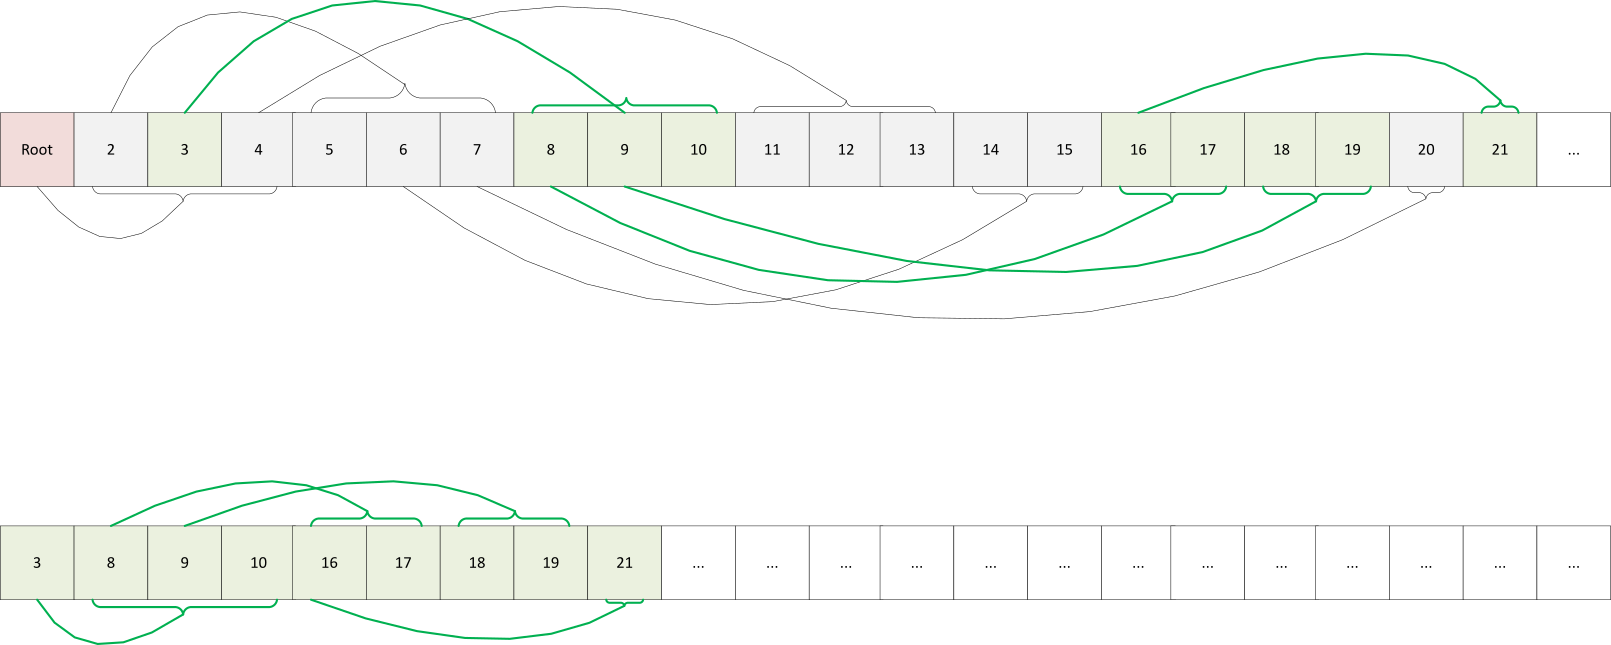
\includegraphics[scale=0.70]{Data_Structure/Working_data/array.png}}
\caption{\label{fig:array}(\textit{Monte Carlo algorithm}).}
\end{figure}


\subsection{Utilities and parameters}
